%!TeX spellcheck = en_EN

\documentclass[12pt]{article}

% Please note that the exam room is given in the Makefile, not here
\newcommand{\coursename}{Example}
\newcommand{\courseacronym}{Ex}
\newcommand{\coursesemester}{SS 17}


\usepackage[a4paper,vmargin={25mm,20mm},hmargin={20mm,25mm}]{geometry}
\usepackage[utf8]{inputenc} 	% Umlaute im Text
\usepackage{xspace}
\usepackage{tabularx}
\usepackage{ltablex}
\usepackage{booktabs}
\usepackage{multicol}
\usepackage{graphicx}
\usepackage[table]{xcolor}

\begin{document}

  \begin{minipage}[c]{4cm}
  
\includegraphics[height=2.5cm,width=\textwidth,keepaspectratio]{../lib/TUC}
  \end{minipage}%
  \hfill%
  \begin{minipage}[c]{4cm}
  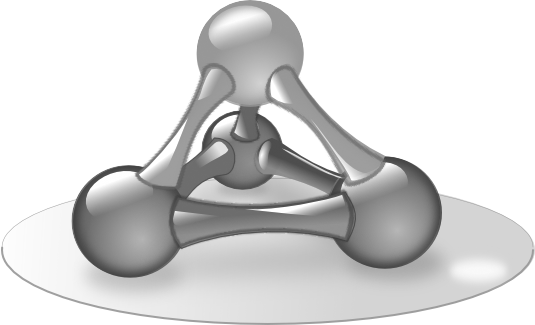
\includegraphics[height=2cm,width=\textwidth,keepaspectratio]{../lib/logo-sw} \\
  {\scriptsize{Professur\\[-2.5mm] Betriebssysteme}\vspace{1mm}}
  \end{minipage}


\begin{centering}
\section*{\coursename \xspace \coursesemester \\ Klausur -- Eingangskontrolle}
\end{centering}

\rowcolors{2}{gray!25}{white}

\begin{tabularx}{\textwidth}{llllr}
\toprule
%  \rowcolor{gray!50}
 Matrikelnummer & Vorname & Nachname & Raum & Platz \\
\midrule
\input{table_withname.tex}
\bottomrule
\end{tabularx}

\end{document}